\section{Identifikation der Reaktionsprodukte} \label{sec:RPMSLeafspray}

Für den Nachweis des Stattfindens der Reaktion der \gls{Chl-K}en mit Essigsäureanhydrid wurde der gleiche Versuchsaufbau wie in Kapitel \ref{sec:Versuchsaufbau} beschrieben verwendet. Das Anhydrid als Reaktionsprodukt konnte durch Verwendung von Acetonitril als \gls{lm} isoliert werden.  

\subsection{Reaktionsprodukt von Bo-DNCC}

Das Reaktionsprodukt von Bo-DNCC konnte mit m/z = 699 [M+K]\textsuperscript{+} bestimmt werden (Strukturvorschlag - Abbildung \ref{fig:699MKstructure}). Identifiziert wurde es über die charakteristische Abspaltung von Essigsäure (M = 60 Da) bei m/z = 639 [M - \ch{CH3COOH} + K]\textsuperscript{+}. Ein Mechanismus für die Abspaltung wird in Abbildung \ref{fig:699MKelectronMovement} vorgeschlagen. Dieser Mechanismus ähnelt dem Mechanismus der Abspaltung von \gls{meoh} (\gls{zB} beobachtbar bei einem Cj-NCC), wie in \cite{StructureElucidation} publiziert.\\

\begin{figure}[!htbp]
  \centering
  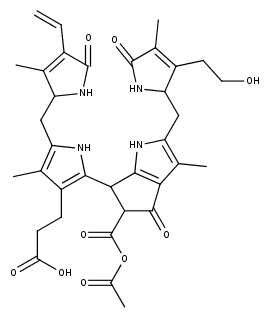
\includegraphics[scale=0.6]{figures/Kapitel4/Kataboliten/fragmentation_structures/VWA_Katabolit_699.png}
  \caption[Strukturvorschlag des Reaktionsproduktes von Bo-DNCC, Quelle: Autor]{Strukturvorschlag des Reaktionsproduktes mit Summenformel \ch{C35H41N4O9}}
  \label{fig:699MKstructure}
\end{figure}

Es wurden Abspaltungen von \ch{H2O} bei m/z = 681 [M - \ch{H2O} + K]\textsuperscript{+}, von \ch{CH3COOH} bei m/z = 639 [M - \ch{CH3COOH} + K]\textsuperscript{+} und von Ring A und Ring D mit \ch{CO2} bei m/z = 311 [M - (Ring A, Ring D, \ch{CO2}) + K]\textsuperscript{+} beobachtet. 

Zur Identifikation der Reaktionsprodukte wurde die \ch{CH3COOH} Abspaltung aufgrund ihrer Dominanz und Eindeutigkeit herangezogen (u. a.
 Abbildung \ref{fig:699MKstructurediags2}). Das Fragment bei m/z = 599 [M - (\gls{nAb}) + K]\textsuperscript{+} ist interessant, da eine Abspaltung von 100 Da bei anderen Kataboliten ebenfalls beobachtet wurde. Die anderen Fragmentierungen in Abbildung \ref{fig:699MKLeafspray} konnten nicht zugeordnet werden. \\

\begin{figure}[!htbp]
  \centering
  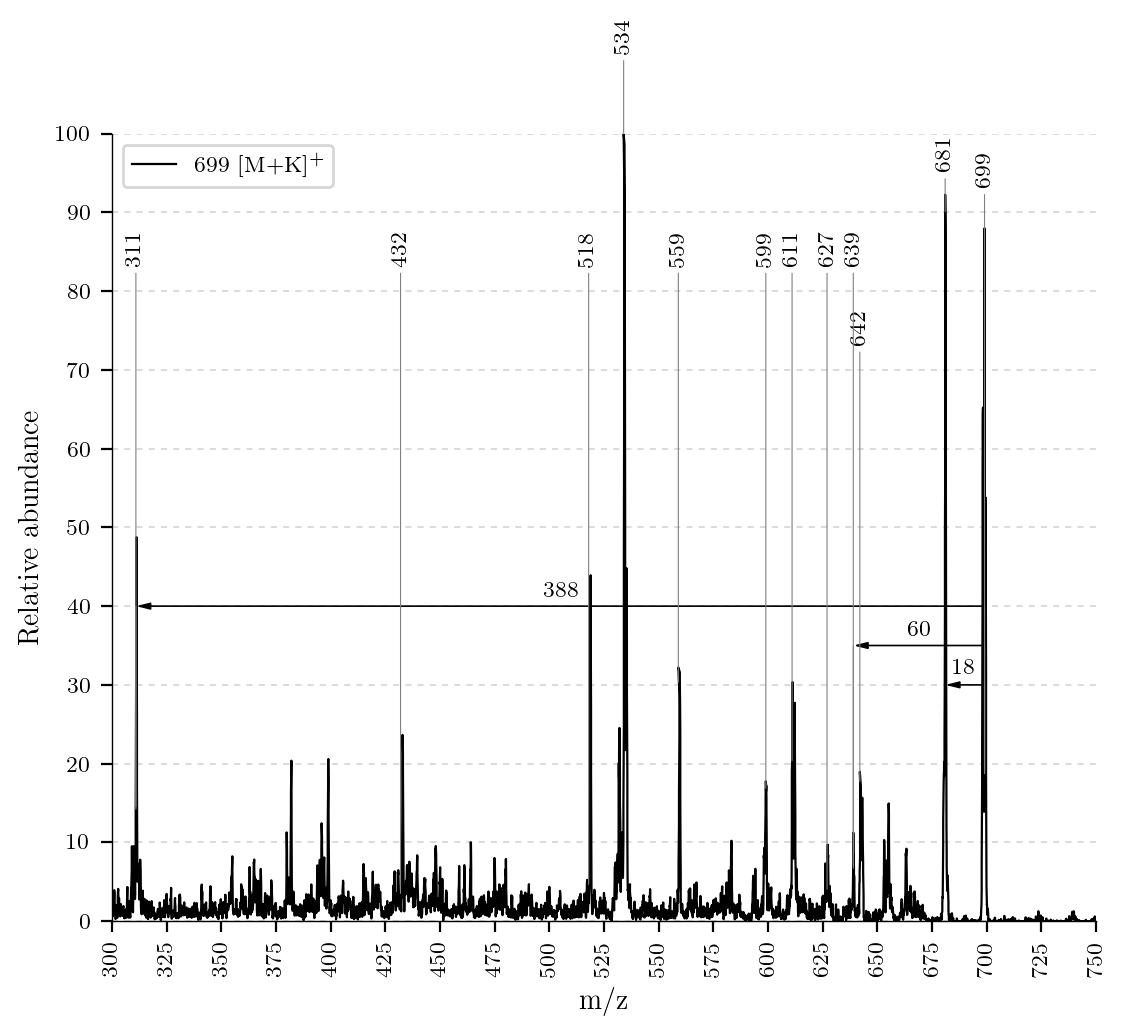
\includegraphics[width=\textwidth, height=0.6\textwidth]{figures/Kapitel4/Kataboliten/VWA_MS_LeafSpray_699.png}
  \caption[ESI-MS Spektrum des Reaktionsproduktes von Bo-DNCC, Quelle: Autor]{ESI-MS Spektrum des Reaktionsproduktes mit m/z = 699 [M+K]\textsuperscript{+}}
  \label{fig:699MKLeafspray}
\end{figure}

Diskussion der Abspaltung bei m/z = 599 [M - (\gls{nAb}) + K]\textsuperscript{+}: Die Abspaltung von 100 Da bei m/z = 599 [M - (\gls{nAb}) + K]\textsuperscript{+} erreicht im Fragmentierungsdiagramm lokale Maxima bei 15 \gls{nKE} und 30 \gls{nKE}. Lokale Minima befinden sich bei 17 \gls{nKE} und 40 \gls{nKE}, an jenen Stellen, an der die Abspaltung von \ch{CH3COOH} lokale Maxima aufweist (Abbildung \ref{fig:699MKstructurediags2}). Daraus könnte man Informationen über den Mechanismus der Abspaltung ableiten. Man könnte sagen, dass die Abspaltung von 100 Da einhergeht mit jener von \ch{CH3COOH} und dass sie mechanistisch miteinander verknüpft sind, also, dass bevor einer Abspaltung des Fragments mit 100 Da \ch{CH3COOH} abgespalten werden muss. Es ließe sich damit erklären, warum bei einem Maximum der einen Abspaltung die andere Abspaltung ein Minimum aufweist.\\ 


\begin{figure}[!htbp]
  \begin{subfigure}[b]{0.5\textwidth}
    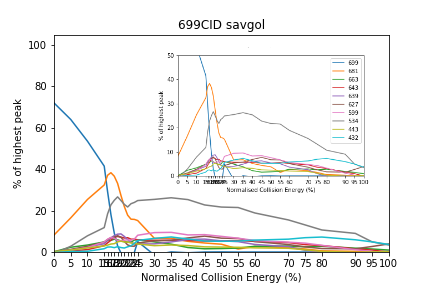
\includegraphics[width=\textwidth, height=\textwidth]{figures/Kapitel4/Kataboliten/diags/699CID-savgol2.png}
    \caption{}
    \label{fig:699MKLeafspraydiags1}
  \end{subfigure}
  \hfill
  \begin{subfigure}[b]{0.5\textwidth}
    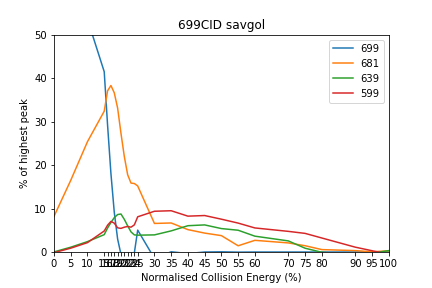
\includegraphics[width=\textwidth, height=\textwidth]{figures/Kapitel4/Kataboliten/diags/699CID-savgol1.png}
    \caption{}
    \label{fig:699MKstructurediags2}
  \end{subfigure}
  
  \caption[Fragmentierungsdiagramme des Reaktionsproduktes von Bo-DNCC, Quelle: Autor]{(a) Fragmentierungsdiagramm des Bo-NCC-3 mit allen beobachteten Abspaltungen (blau = 699 [M+K]\textsuperscript{+}, orange = 681 [M - \ch{H2O} + K]\textsuperscript{+}, grün = 663 [M - (2x\ch{H2O}) + K]\textsuperscript{+}, rot = 643 [M - (\gls{nAb}) + K]\textsuperscript{+}, violett = 639 [M - \ch{CH3COOH} + K]\textsuperscript{+}, braun = 627 [M - (\gls{nAb}) + K]\textsuperscript{+}, pink = 599 [M - (\gls{nAb}) + K]\textsuperscript{+}, grau = 534 [M - (\gls{nAb}) + K]\textsuperscript{+}, hellgrün = 443 [M - (\gls{nAb}) + K]\textsuperscript{+}, türkis = 432 [M - (\gls{nAb}) + K]\textsuperscript{+}), (b) Fragmentierungsdiagramm mit ausgewählten Abspaltungen (blau = 699 [M+K]\textsuperscript{+}, orange = 681 [M - \ch{H2O} + K -\ch{H2O}, grün = 639 [M - \ch{CH3COOH} + K], rot = 599 [M - (\gls{nAb}) + K]\textsuperscript{+})}
\end{figure} 

Im Fragmentierungsdiagramm erreicht die \ch{H2O} Abspaltung ein lokales Maximum bei 17 \gls{nKE}. Die Abspaltung nimmt bis zu 30 \gls{nKE} stark ab und bleibt bis zu 90 \gls{nKE} erhalten. Im Vergleich zum Fragmentierungsdiagramm des nicht reagierten Bo-DNCC erfolgt die \ch{H2O} Abspaltung bei einer niedrigeren \gls{nKE} und ist länger beobachtbar (vergleiche Abbildungen \ref{fig:619MKLeafspraydiags} und \ref{fig:699MKstructurediags2}). Es gilt zu bedenken, dass beim nicht reagierten Bo-DNCC das [M+H]\textsuperscript{+}-Ion aufgenommen wurde, wohingegen man beim reagierten Bo-DNCC das [M+K]\textsuperscript{+}-Ion analysierte. Der Unterschied im Verlauf der Kurven könnte somit auch durch diesen Umstand hervorgerufen werden.

Die Abspaltung von \ch{CH3COOH} besitzt lokale Maxima bei 20 \gls{nKE} und 45 \gls{nKE}. Das Maximum bei 45 \gls{nKE} ist weniger intensiv. Die Intensität der Abspaltung nimmt dabei kontinuierlich bis zu einer von 80 \gls{nKE} ab (Abbildung \ref{fig:699MKstructurediags2}). Ein lokales Minimum der Abspaltung befindet sich zwischen 23 \gls{nKE} und 30 \gls{nKE}. \\



\begin{figure}[!htbp]
  \begin{subfigure}[b]{0.5\textwidth}
    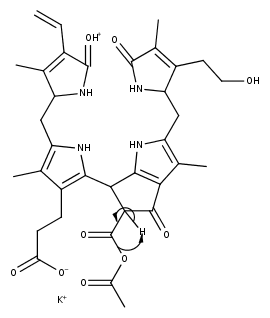
\includegraphics[width=\textwidth, height=\textwidth]{figures/Kapitel4/Kataboliten/fragmentation_structures/VWA_Katabolit_699-639_MK_electronMovement.png}
    \caption{}
    \label{fig:699MKelectronMovement}
  \end{subfigure}
  \hfill
  \begin{subfigure}[b]{0.5\textwidth}
    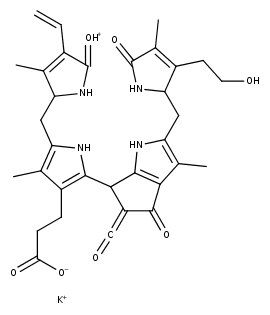
\includegraphics[width=\textwidth, height=\textwidth]{figures/Kapitel4/Kataboliten/fragmentation_structures/VWA_Katabolit_699-639_MK.png}
    \caption{}
    \label{fig:699MK639}
  \end{subfigure}
  \caption[Vorschlag des Mechanismus der \ch{CH3COOH} Abspaltung, Quelle: Autor]{(a) vorgeschlagener Mechanismus der Essigsäureabspaltung und (b) das Produkt, wobei \ch{CH3COOH} als stabiles Neutralteilchen abgespalten wird}
\end{figure}



\pagebreak
\subsection{Reaktionsprodukt von Bo-NCC-3}

Die Molekülmasse des Reaktionsproduktes von Bo-NCC-3 konnte mit m/z = 727 [M+K]\textsuperscript{+} bestimmt werden. Eine Abspaltung von Essigsäure wurde bei m/z = 667 [M+K]\textsuperscript{+} beobachtet. Weiters wurde eine Abspaltung von \ch{H2O} bei m/z = 709 [M - \ch{H2O} + K]\textsuperscript{+} beobachtet. Bei der Abspaltung bei m/z = 627 [M - (\gls{nAb}) + K]\textsuperscript{+} könnte es sich um die gleiche Abspaltung wie beim Reaktionsprodukt des Bo-DNCC handeln, da auch ein Fragment mit M = 100 Da abgespalten wird. Die anderen Abspaltungen (Abbildung \ref{fig:727MKLeafspray}) konnten nicht eindeutig zugeordnet werden.

\begin{figure}[!htbp]
  \centering
  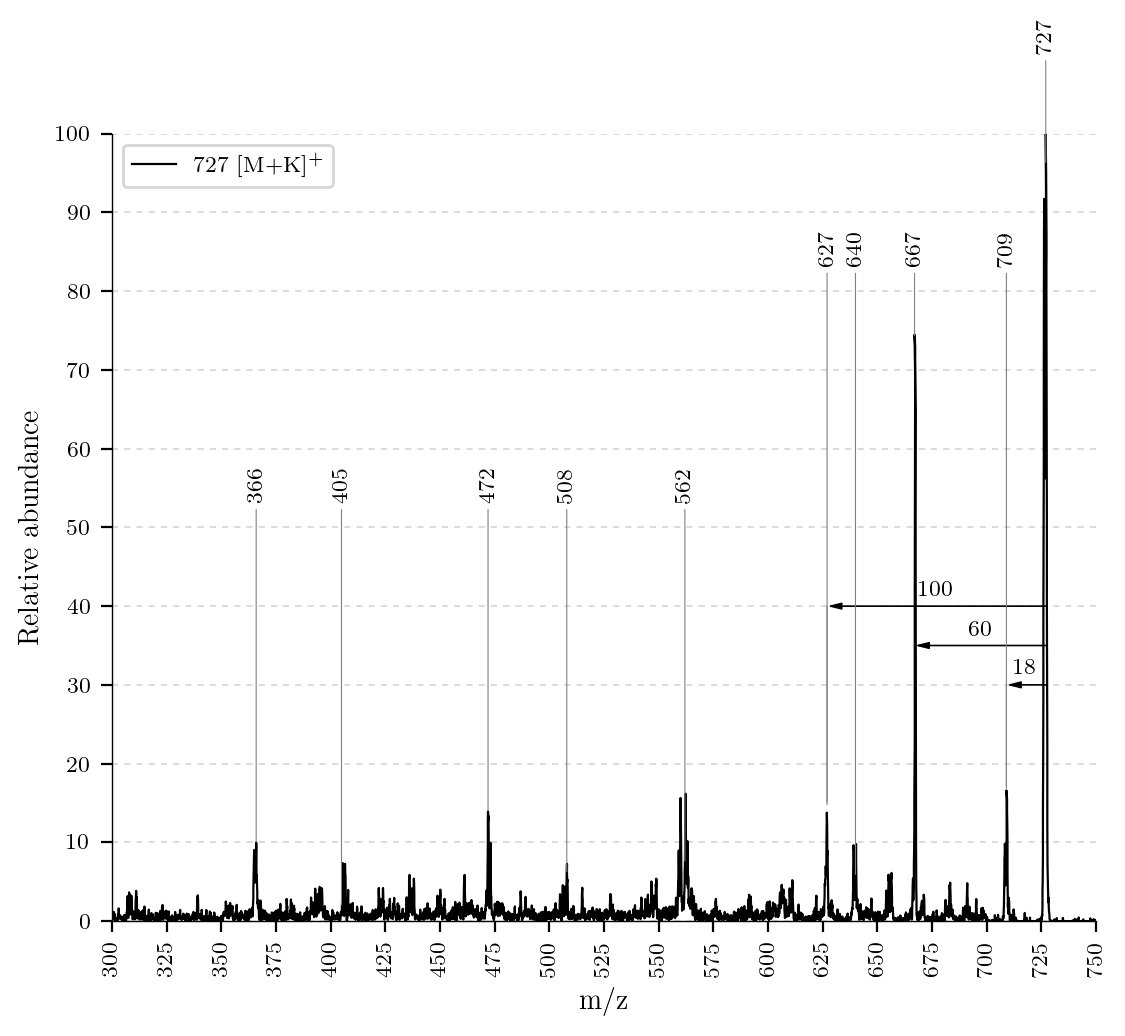
\includegraphics[width=\textwidth, height=0.7\textwidth]{figures/Kapitel4/Kataboliten/VWA_MS_LeafSpray_727.png}
  \caption[ESI-MS des Reaktionsproduktes von Bo-NCC-3, Quelle: Autor]{ESI-MS Spektrum des Reaktionsproduktes bei m/z = 727 [M+K]\textsuperscript{+}}
  \label{fig:727MKLeafspray}
\end{figure}

\begin{figure}[!htbp]
  \centering
  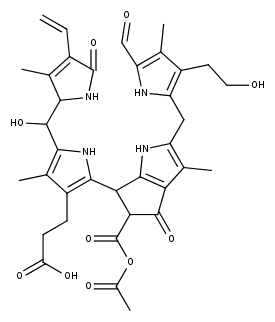
\includegraphics[scale=0.6]{figures/Kapitel4/Kataboliten/fragmentation_structures/VWA_Katabolit_727.png}
  \caption[Strukturvorschlag des Reaktionsproduktes von Bo-NCC-3, Quelle: Autor]{Strukturvorschlag des Reaktionsproduktes mit Summenformel \ch{C36H40N4O10}}
  \label{fig:727MKstructure}
\end{figure}

Es wurde beobachtet, dass die Abspaltung von \ch{H2O} bei niedrigeren Energien erfolgt wie jene von \ch{CH3COOH}. Im Vergleich zum Fragmentierungsdiagramm des Reaktionsproduktes des Bo-DNCC (Abbildung \ref{fig:699MKLeafspraydiags1}) kann als Charakteristikum der \ch{CH3COOH} Abspaltung ein lokales Maximum bei 45 \gls{nKE} gedeutet werden (Abbildung \ref{fig:699MKstructurediags2} und Abbildung \ref{fig:727MKLeafspraydiags}). Die Abspaltung von \ch{H2O} weist bei beiden Kataboliten ein lokales Maximum bei 15 \gls{nKE} auf und besitzt einen ähnlichen Kurvenverlauf (Abbildung \ref{fig:699MKstructurediags2} und Abbildung \ref{fig:727MKLeafspraydiags}). Dies lässt darauf schließen, dass es sich bei dieser \ch{H2O}-Abspaltung um eine Abspaltung auf ein und dersselben Position handelt. Als Position der Abspaltung wird die Hydroxygruppe an Position 32 des Chl-Kataboliten vorgeschlagen. 

\begin{figure}[!htbp]
  \centering
  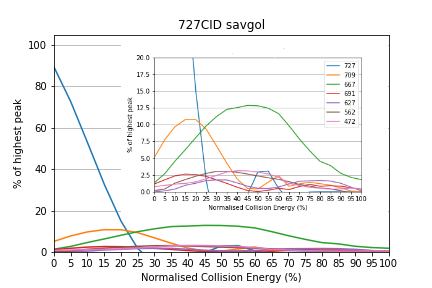
\includegraphics[scale=0.7]{figures/Kapitel4/Kataboliten/diags/727CID-savgol.png}
  \caption[Fragmentierungsdiagramm des Reaktionsproduktes von Bo-DNCC, Quelle: Autor]{Fragmentierungsdiagramm des Reaktionsproduktes (blau = 727 [M+K]\textsuperscript{+}, orange = 709 [M - \ch{H2O} + K]\textsuperscript{+}, grün = 667 [M - \ch{CH3COOH} + K]\textsuperscript{+}, rot = 691 [M - ? + K]\textsuperscript{+}, violett = 627 [M - ? + K]\textsuperscript{+}, braun = 562 [M - ? + K]\textsuperscript{+}, pink = 472 [M - ? + K]\textsuperscript{+})}
  \label{fig:727MKLeafspraydiags}
\end{figure}



\subsection{Reaktionsprodukt von Bo-NCC-1}

Erwartungsgemäß konnte das Reaktionsprodukt des Bo-NCC-1 bei m/z = 873 [M+K]\textsuperscript{+} gefunden werden. Es zeigt Abspaltungen von \ch{H2O} bei m/z = 855 [M - \ch{H2O} + K]\textsuperscript{+}, von Essigsäure bei m/z = 813 [M - \ch{CH3COOH} + K]\textsuperscript{+}und von \ch{CH3COOH}, Ring A, Ring D, zweimal \gls{meoh} und \ch{CO} bei m/z = 309 [M - (Ring A, Ring D, 2mal MeOH, \ch{CO})  + K]\textsuperscript{+} (diesselbe Abspaltung wurde beim Reaktionsprodukt m/z = 661 [M+H]\textsuperscript{+} beobachtet - Kapitel \ref{sec:ESIMSRPBoNCC3}). Beim Fragment m/z = 441 [M - (Ring D, 2mal MeOH, \ch{H2O}) + K]\textsuperscript{+} könnte es sich um eine Abspaltung von Ring D, zweimal \gls{meoh} und \ch{H2O} handeln. 

\begin{figure}[htbp]
  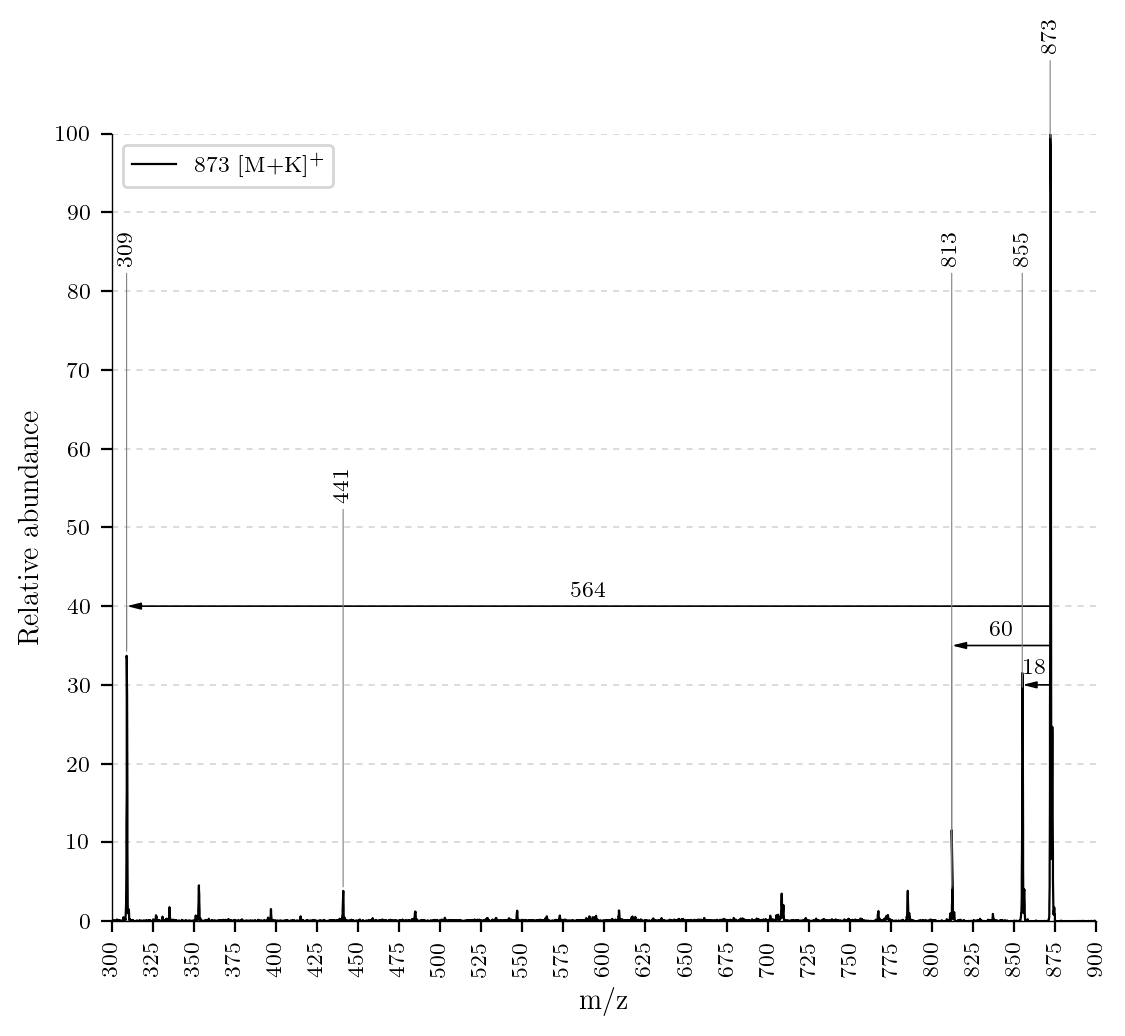
\includegraphics[width=\textwidth, height=0.7\textwidth]{figures/Kapitel4/Kataboliten/VWA_MS_LeafSpray_873.png} 
  \caption[ESI-MS des Reaktionsproduktes von Bo-NCC-1, Quelle: Autor]{ESI-MS des Reaktionsproduktes bei m/z = 873 [M+K]\textsuperscript{+}}
  \label{fig:873MKLeafspray}
\end{figure}

\begin{figure}[htbp]
  \centering
  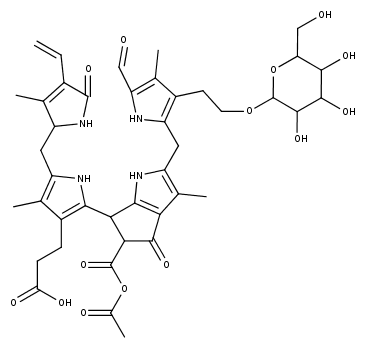
\includegraphics[scale=0.6]{figures/Kapitel4/Kataboliten/fragmentation_structures/VWA_Katabolit_873.png}
  \caption[Strukturvorschlag des Reaktionsproduktes von Bo-NCC-1, Quelle: Autor]{Strukturvorschlag des Reaktionsproduktes mit Summenformel \ch{C42H50N4O14}}
  \label{fig:873MKstructure}
\end{figure}

Im Fragmentierungsdiagramm sieht man, dass sich das lokale Maximum der Essigsäureabspaltung hin zu niedrigeren Energien verschoben hat. Es befindet sich nun bei  35 \gls{nKE}. Auch die \ch{H2O} Abspaltung verschiebt sich zu niedrigeren Energien und besitzt ein lokales Maximum bei 10 \gls{nKE}. Im Vergleich zum Bo-DNCC und Bo-NCC-3 nahmen diese Werte um 10 bzw. 5 Einheiten an \gls{nKE} ab. Dieser Zusammenhang wurde in zwei voneinander unabhängigen Experimenten beobachtet (Abbildung \ref{fig:873MKLeafspraydiags1} und Abbildung \ref{fig:873MKstructurediags2}). Die Ursache könnte beim Zuckerring liegen, der die Elektronenverteilung vermutlich so beeinflusst, dass die Abspaltungen bereits bei niedrigeren Energien erfolgen. 

(Einfügen von 3D Bildern, die die sterischen Zusammenhänge vorschlagen).


\begin{figure}[!htbp]
  \begin{subfigure}[b]{\textwidth}
    \centering
    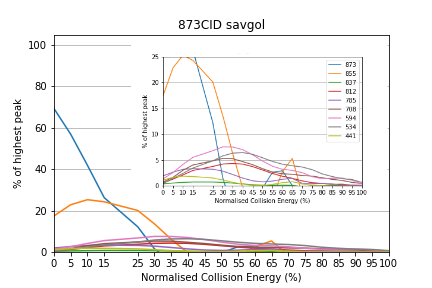
\includegraphics[scale=0.9]{figures/Kapitel4/Kataboliten/diags/873CID-savgol1.png}
    \caption{}
    \label{fig:873MKLeafspraydiags1}
  \end{subfigure}
  \hfill
  \begin{subfigure}[b]{\textwidth}
    \centering
    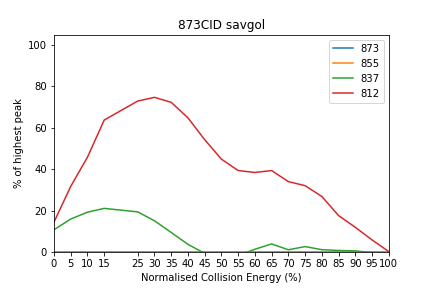
\includegraphics[scale=0.9]{figures/Kapitel4/Kataboliten/diags/873CID-savgol2.png}
    \caption{}
    \label{fig:873MKstructurediags2}
  \end{subfigure}
  
  \caption[Fragmentierungsdiagramm des Reaktionsproduktes von Bo-NCC-1, Quelle: Autor]{Fragmentierungsdiagramm des Reaktionsproduktes: (a) Experiment am 13.09.2017 (11:00) - (blau = 873, orange = 855, grün = 837, rot = 812, violett = 765, braun = 708, pink = 594, grau = 534, hellgrün = 441), (b) Experiment am 13.09.2017 (09:45) - schlechter gelungen, weswegen die Abspaltungen nicht so schön wie in Experiment (a) zu sehen sind (blau = 873, orange = 855, grün = 837, rot = 812)}
\end{figure}